\chapter{Installation, Commissioning, and Maintenance Instructions for Alternating Current Motors}

\begin{figure}[ht]
    \centering
    
\includegraphics[width=0.1\linewidth]{images/page_62_manufacturer_logo}
    \label{fig:alternating_motor_manufacturer_logo}
\end{figure}

{\small

\section*{1. Installation}

The installation of motors depends on the conditions in which they are intended to operate.
Normal-type, \textbf{protected, ventilated} motors should only be installed in dry and non-dusty areas.
\textbf{Special insulation motors} should be used in areas where water condensation, dust, or aggressive gases may occur.
For operations where our standard motors are not suitable, we have developed special types (motors with a protective cap against water droplets,
    enclosed motors with or without fresh air intake, etc.).

During installation, consideration should be given to the accessibility of parts that may require periodic inspection,
    such as bearings, brushes, terminal plate, short-circuit device, etc.

It is advisable to mount the motor on a concrete base, directly or on slides.
The rotor axis, especially for motors with plain bearings and lubrication by rings, \textbf{must be perfectly horizontal and parallel to the shaft it is intended to drive.}

If the motor is mounted on slides, it is better to first screw them onto the motor, then place the assembly on the base,
    place shims under the slides, and finally seal them.
When the installation is complete, tighten the motor fixing screws to the slides or base, taking care not to twist the motor frame.

In the case of \textbf{belt drive}, the center of the motor pulley and the driven pulley must be perfectly in the same plane.
The belt should not be too tight, otherwise, the bearings would be subject to excessive pressure and could \textbf{overheat}.

\textbf{Ball bearing motors} can be mounted against a wall or ceiling, even in a vertical or inclined position if necessary,
    provided that, apart from the weight of the pulley or coupling, the motor shaft is not subject to any other axial force.

In such cases, the bearing flanges of \textbf{ring-lubricated motors} must be turned 90° or 180° so that the oil filling opening is always at the top.

The motor shaft ends are machined according to the \textbf{VSM tolerance system} (Swiss Society of Machine Builders),
    \textbf{light pressed fit k5}, and equipped with a keyway with a key according to VSM standards.
The parts to be mounted on the shaft ends must have a normal H6 bore.
This adjustment has been adopted because the forcing resulting from a tight fit easily causes excessive axial loads on the bearings.
The faces of the shaft ends are drilled with a threaded hole (see figures 3 and 4) to allow the axial fixing
of transmission components such as pulleys, gears, couplings, etc., with a washer and screw.

The installation of pulleys, gears, couplings, etc., on the shaft ends is done using a screw inserted into the threaded
hole and an appropriate device. When pulleys, etc., are not supplied by us, care should be taken to ensure that they are carefully balanced.

\section*{2. Connection}

Before connecting the motor, check if the voltage indicated on the nameplate matches the network voltage.
Connect the motor according to the instructions on the diagram supplied with the motor or attached inside the terminal cover.
Grounding is done by the yellow screw.

    \begin{wrapfigure}{R}{0.35\textwidth}
        \centering
        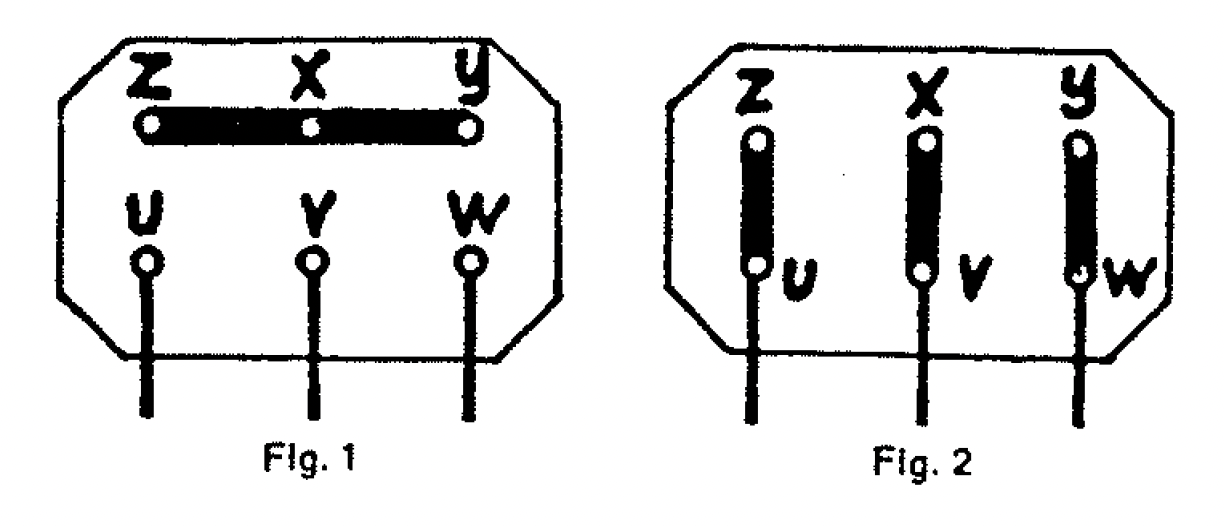
\includegraphics[width=0.33\textwidth]{images/page_62_alternating_motor_connections}
        \label{fig:alternating_motor_connections}
    \end{wrapfigure}

    The motor stator typically has a terminal plate with 6 terminals to which the phase arrivals and departures are connected.
    If it is a three-phase motor designed for two voltages E and E V3,
    connections should be made as indicated in Figure 1 for the higher voltage (star connection) and,
    for the lower voltage (delta connection), according to Figure 2.

\section*{3. Rotation Direction}

To reverse the rotation direction, simply swap two of the current leads at the stator terminals;
for three-phase motors: two current leads, for biphasic motors with compound voltage: the two outer conductors,
    for biphasic motors with non-compound voltage and single-phase motors: two current leads from the same phase.
    If the motor is equipped with a double-width pulley for driving a fixed pulley and idle pulley, the belt must be on the idle pulley at startup.
The belt should be brought onto the fixed pulley only when the motor has reached its full speed.
Unless the motor has a third bearing (external), the belt must always rotate on the bearing flange side.
If the motor stops for any reason, it must be immediately switched off to prevent damage.
Maximum temperatures: bearings, about 50\textdegree C; windings and iron, 80\textdegree C above ambient temperature (max. 40\textdegree C).

\section*{4. Maintenance}

All our \textbf{ball bearing motors} are supplied with enough grease to last approximately 6 to 12 months under normal operating conditions.
A good ball bearing grease should be used, which will be pumped into the bearings using Stauffer or Técalémit "S" grease fittings (figure 3).


    \begin{wrapfigure}{L}{0.35\textwidth}
        \centering
        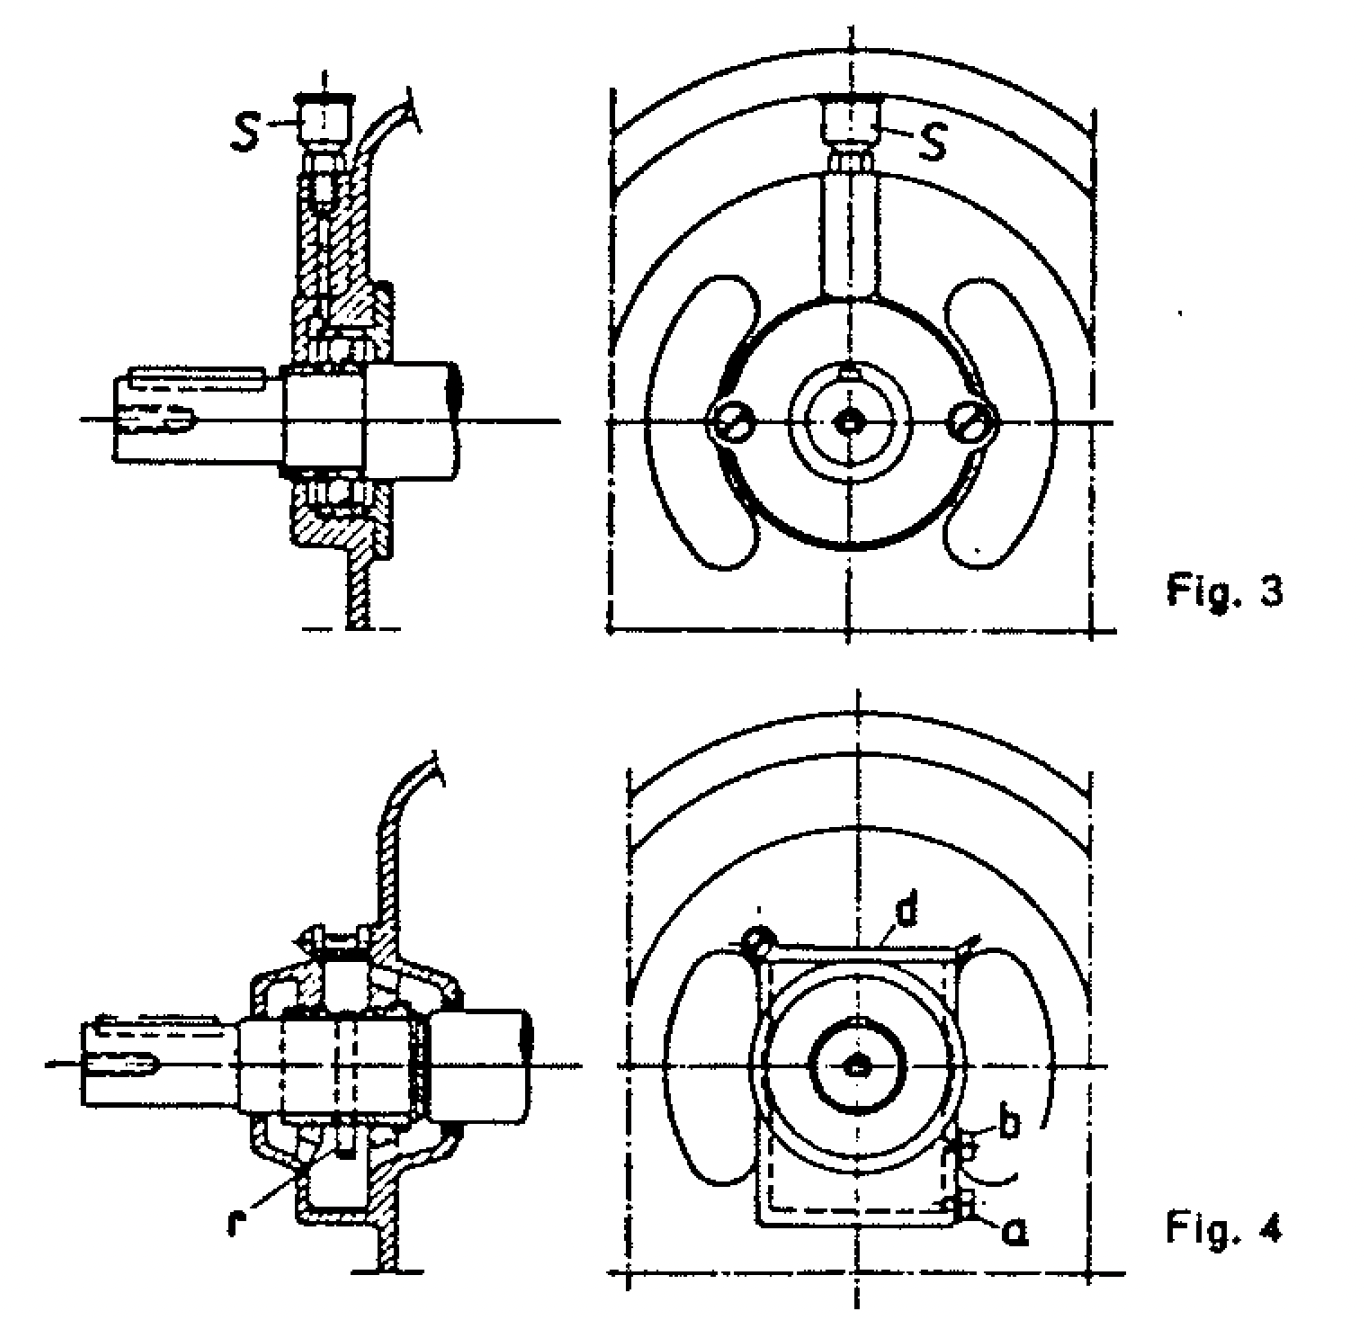
\includegraphics[width=0.33\textwidth]{images/page_62_maintenance}
        \label{fig:alternating_motor_maintenance}
    \end{wrapfigure}

    \textbf{Bearing ring motors} are shipped without oil.
    Before commissioning, it is recommended to clean the oil chambers with gasoline and, when dry, fill them with resin- and acid-free machine oil.
This initial oil charge will be renewed about 1 month later and then again 2 to 4 months later.
Afterward, the oil should be changed every 6 months. To do this, drain the oil by removing screw "a" (Figure 4) and clean the oil chamber with gasoline. Then, replace screw "a," loosen screw "b," and pour in new oil until it overflows through overflow "b." Replace screw "b" and close the bearing cover.

It is absolutely essential that the oil feed ring "r" comes with the shaft and transports oil. Periodically check its condition and purity.

For \textbf{motors with ring-induced}, occasionally check if the rings are still smooth and free of carbon dust. Spark production can result from ovalization of the rings, burns, improper brush support, insufficient brush pressure, brushes or support rods having play, or vibrations due to improper motor installation.

If the rings are only slightly ovalized, burned, or dirty, simply sand them with emery or glass paper using a wooden piece that matches the curvature of the rings. If the rings are considerably damaged, it will be necessary to grind and then polish them on a lathe. Never apply paraffin, grease, etc., to the rings.

If the brushes do not press with their entire surface on the rings, they should be sanded by placing a piece of emery cloth on the rings and moving it back and forth under the brushes until the contact surface of each brush perfectly matches that of the ring.

Carefully remove carbon and metal particles, dust, etc., and wipe the rings with a dry cloth. Repeat the same process when installing new brushes. Since bronze brushes are relatively hard, it is preferable to give them a curvature corresponding to that of the rings using a half-round file, and then finish this work with emery cloth. Slightly chamfer the edges of the brushes to avoid spark production at these points.

The wear of brushes and rings in \textbf{fixed-brush} motors is naturally higher than in motors with \textbf{ring short-circuiting and brush lifting devices}. Always keep the short-circuiting contacts of the rings and the rotor starter clean and lightly grease them with Vaseline. Remove any fusion beads that may occur using a file and emery paper.

\section*{5. Spare Parts}

When ordering spare parts such as bearings, plain bearings, brush holders, brushes, etc., it is essential to specify the manufacturing number and type of the motor found on the nameplate. In case of doubt (especially for older motors), send a model of the desired part to the factory.

Replacement brushes must absolutely be of the same brand as those delivered with the motor. When ordering brushes, also specify their brand and dimensions (for example, SR 81, 16 x 32 mm). In case of disputes, it is better to send a few used brushes to our factory, as their appearance often helps identify the cause of the disputes.

}